% Project DAD (Data Anomaly Detection) Console technical whitepaper -- Overleaf source.
% Upload this file with the folder figures/ (the user-guide screenshots, JPEG) beside it,
% and select this file as the Main document. Compiler: pdfLaTeX.
% No bibliography files, shell escape or custom fonts required.
% Compile twice to resolve the table of contents, citations and cross-references.
% The appendices are a separate document, TECHNICAL_WHITEPAPER_APPENDICES.tex, compiled on its own.
% Simplified core edition. Detailed methods, user guide and supporting results are in the companion appendices.
\documentclass[11pt,a4paper]{article}
\usepackage[T1]{fontenc}
\usepackage[utf8]{inputenc}
\usepackage{lmodern}
\usepackage[margin=24mm,headheight=15pt]{geometry}
\usepackage{microtype}
\usepackage{amsmath,amssymb}
\usepackage{booktabs,longtable,array,ragged2e}
\usepackage[table]{xcolor}
\usepackage{graphicx}
\usepackage[section]{placeins}
\usepackage{float}
\usepackage{tikz}
\usetikzlibrary{arrows.meta,positioning,calc}
\usepackage{enumitem}
\usepackage{titlesec}
\usepackage{fancyhdr}
\usepackage{caption}
\usepackage{xurl}
\usepackage{hyperref}
\usepackage{bookmark}

\definecolor{ink}{HTML}{183348}
\definecolor{accent}{HTML}{236578}
\definecolor{pale}{HTML}{EDF3F6}
\definecolor{reviewred}{HTML}{B42318}
\hypersetup{colorlinks=true,linkcolor=ink,citecolor=accent,urlcolor=accent,
  pdftitle={Project DAD (Data Anomaly Detection) Console: Towards Proactive Monitoring by Discovering Early Signs of Incidents in Server Logs},
  pdfsubject={Technical whitepaper: local log analysis, anomaly detection, sequential pattern mining and investigation}}
\urlstyle{tt}
\setlength{\parindent}{0pt}
\setlength{\parskip}{0.55em}
\setlength{\emergencystretch}{3em}
\setlength{\tabcolsep}{5pt}
\renewcommand{\arraystretch}{1.22}
\setlength{\LTpre}{0.8em}
\setlength{\LTpost}{0.8em}
\setlength{\LTleft}{0pt}
\setlength{\LTright}{0pt}
\captionsetup{font=small,labelfont=bf,skip=8pt}
\titleformat{\section}{\Large\bfseries\color{ink}}{\thesection.}{0.6em}{}
\titleformat{\subsection}{\large\bfseries\color{ink}}{\thesubsection.}{0.6em}{}
\titlespacing*{\section}{0pt}{1.5em}{0.6em}
\titlespacing*{\subsection}{0pt}{1.0em}{0.4em}
\setcounter{tocdepth}{2}
\pagestyle{fancy}
\fancyhf{}
\fancyhead[L]{\small\textsc{Project DAD Console}}
\fancyhead[R]{\small Technical whitepaper}
\fancyfoot[C]{\small\thepage}
\renewcommand{\headrulewidth}{0.3pt}
\setlist{nosep,leftmargin=*}

% Project files are repository-relative provenance, not files required by LaTeX.
% Their paths are printed so the paper remains meaningful when moved to Overleaf.
\newcommand{\projectref}[2]{#1 {\footnotesize(\nolinkurl{#2})}}
\graphicspath{{figures/}}
% A literal token or short phrase in typewriter type; spaces are kept, unlike \nolinkurl.
\newcommand{\tok}[1]{\texttt{\detokenize{#1}}}
% A user-guide screenshot: file name, width as a fraction of the text width, caption, label.
\newcommand{\screenshot}[4]{\begin{figure}[H]\centering
  \fbox{\includegraphics[width=#2\linewidth,keepaspectratio]{#1}}
  \caption{#3}\label{#4}\end{figure}}
\setlength{\fboxsep}{0pt}
\setlength{\fboxrule}{0.4pt}

\begin{document}
% Number the title page A so its PDF anchor does not clash with arabic page 1.
\pagenumbering{Alph}
\begin{titlepage}
\thispagestyle{empty}
{\small\sffamily\color{accent} TECHNICAL WHITEPAPER\par}
\vspace{1.8cm}
{\Huge\bfseries\color{ink} Project DAD\par}
\vspace{0.3cm}
{\Large\bfseries\color{ink} (Data Anomaly Detection) Console\par}
\vspace{0.7cm}
{\LARGE\bfseries Towards Proactive Monitoring: Discovering Early Signs of Incidents in Server Logs\par}
\vspace{1.0cm}
{\large 26 October 2026\par}
\vspace{1.6cm}
\textbf{Implementation baseline:} application release 0.2.0 plus the current workspace inspected on 26 October 2026, including sequential pattern mining, pattern discovery, user whitelisting, frozen-runtime operation, Sigma rules as a fifth detector, a customisable Dashboard, a separate SQL password and a hardened local service; a parser for a fifth source, fixed-width event logs, is in progress. These are implemented in the current source; none is a new numbered release. This edition restates the project's motivation and goals; it reports no new experiment.
\vfill
{\small Repository paths identify supporting project evidence; those files are not needed to compile this document. The companion user-guide screenshots are in \nolinkurl{whitepaper/figures/}.}
\end{titlepage}
\pagenumbering{roman}

\section*{Executive Summary}
\addcontentsline{toc}{section}{Executive Summary}

Project DAD (Data Anomaly Detection) Console is a small part of a wider effort to move cybersecurity monitoring from reacting to incidents towards discovering signs that an incident may develop. It learns what normal activity looks like from historical server logs, ranks observations that depart from it and presents each one, with its evidence, for human review.

The project has three goals. The \textbf{ultimate goal} is proactive discovery: surfacing rare patterns and anomalous behaviour early enough to prepare for extraordinary events that need immediate attention. The \textbf{secondary goal} is to rely less on static rules, which take time to develop and implement and cover only what someone already anticipated; DAD's baselines, thresholds and routines are learned from the data. The \textbf{tertiary goal} is to establish the baselines, review records and labels that a future malicious/benign classifier will need. An \textbf{added benefit} is rule discovery: in the best case, a finding can be traced back to the chain of events behind it, and chains that recur can be developed into rules, including rules a person would not recognise or think to write.

Two conditions qualify this approach. First, rare is not the same as unexplained: cases that have already been recorded and accepted, such as a vouched-for service account, must be recognised rather than raised again. The console's audited user whitelist does this after scoring. Second, the detectors know nothing of the organisation's accounts, systems, maintenance or changes. Their findings need integration with a rule-based or agentic context layer that removes likely false positives before they reach an analyst. That layer is planned; today a reviewer supplies the context.

The immediate priority is to explain what has already been flagged. For each anomalous group, analysts draft competing benign and malicious hypotheses, each with the test that would refute it. A group is resolved by a review label, or by a scoped whitelist entry when a named account explains it. A first register holds 32 groups and 91 hypotheses. Automated machine learning (AutoML) is a natural extension once those labels exist.

The current application parses supported logs, builds several observation views, applies complementary anomaly detectors, discovers common event sequences and presents findings for review. Simple mode follows four steps: \textbf{Upload, Analyze, Map and Review}. Reports retain evidence and decisions in versioned cases.

Historical processing covered approximately 26.3 million lines from AUTH, OSSEC, PF and IPFilter. In the recorded AUTH test view, sequence scoring produced 608 candidate sessions, including 192 not flagged by the other three mechanisms in the Dashboard comparison; none of these candidates required a hand-written rule. This demonstrates complementary prioritisation, not validated attack recall or early warning. The project does not yet have an independently adjudicated attack/benign dataset from which to establish detection accuracy, lead time or measured analyst savings.

The original historical corpus has been purged from the current workspace. A frozen runtime preserves inference artifacts and maps so that new supported uploads can still be analysed; it cannot reconstruct historical raw evidence. Uploaded excerpts retain their own review context.

The justified next step is a governed analyst-assisted pilot: work through the hypothesis register with server owners and change records, verify findings against independently reviewed data, measure whether and how early flagged observations precede incidents or operational problems, connect a first context layer, measure review effort and collect quality-controlled labels for the classifier. The companion appendices preserve the detailed methods, user guide, implementation record and supporting results.

\clearpage
\tableofcontents
\clearpage
\pagenumbering{arabic}

\section{Introduction and Practical Motivation}

\subsection{From Reacting to Anticipating}

Most monitoring is reactive. An incident is recognised once it matches a known signature, causes visible disruption or is reported, and the response starts from that point. Moving towards proactivity means looking for weaker signals earlier: activity that is rare for a host, an account that has not been seen before, an unusual order of events or a monitoring agent that falls silent. Each signal is a reason to look, not a conclusion. Many will be benign changes; a few may be the early stages of an event that needs immediate attention.

Project DAD Console is a small part of a wider effort towards proactive monitoring. Its role is to learn normal behaviour from local server logs, rank what departs from it and keep each finding connected to its evidence and to a person's judgement.

\subsection{Goals}

Table~\ref{tab:core-goals} states the project's three goals, an added benefit, and what the current implementation contributes to each.

\begin{table}[H]
\centering\small
\begin{tabular}{p{0.12\linewidth}p{0.36\linewidth}p{0.43\linewidth}}
\toprule
\textbf{Goal} & \textbf{Aim} & \textbf{Current contribution} \\
\midrule
Ultimate & Discover signs that an incident may happen, rather than only respond once it has. & Unsupervised detectors rank rare and anomalous behaviour against baselines learned from a year of logs. \\
Secondary & Rely less on static rules, which take time to develop and implement. & Baselines, thresholds and frequent routines are learned from data; reviewed routines can be proposed as candidate rules. \\
Tertiary & Establish the baselines and systems for a future malicious/benign classifier. & Frozen baselines, five review dispositions, versioned reports and Phase~8 label-preparation scaffolding; no classifier is trained yet. \\
Added benefit & Discover rules: trace findings back to the chains of events behind them and develop recurring chains into rules. & 53 AUTH and 81 OSSEC sequential rules and frequent routines mined from training data, alert profiles and named unusual transitions; none adopted as an operational rule. \\
\bottomrule
\end{tabular}
\caption{Project goals and an added benefit. The contributions are capabilities; none is yet measured against incidents.}
\label{tab:core-goals}
\end{table}

Moving away from static rules does not mean discarding them. A rule encodes known context, such as an approved maintenance account or a permitted address range, cheaply and transparently. The limitation is that a rule describes only what someone already expected, and writing, approving and implementing it takes time. Learned baselines can notice what nobody wrote a rule for; rules remain the natural way to state context that is already known.

The two approaches can also feed each other. Rules written by people tend to follow a heuristic, a guideline or a recognisable pattern, such as repeated failed logins within a minute. Mining the data has no such preference, so it can surface regularities that are not obvious or intuitive to a person. Rule discovery (Section~\ref{sec:core-rules}) turns such regularities into candidate rules for review.

\subsection{Recorded Cases and Missing Context}

Searching for the rare has two consequences that the design must address.

\textbf{Recorded cases.} Rare does not mean unexplained. Some rare activity has already been examined and accepted: a service account that runs once a month, or a named administrator who works on an unusual host. Raising it again each time spends review effort without adding information. The console records such cases as audited user whitelist entries applied after scoring (Section~\ref{sec:core-whitelist}); covered observations stay scored and visible but stop requesting attention. Recorded cases come from testing hypotheses about each flagged group (Section~\ref{sec:core-hypotheses}).

\textbf{Missing context.} The detectors see only the logs. They do not know who owns an account, which systems were in maintenance, which changes were approved or which addresses belong to partners. A statistically unusual observation can be entirely expected to someone who holds that context. The detection layer therefore needs integration with a rule-based or agentic layer that brings in this context and removes likely false positives before findings reach an analyst (Section~\ref{sec:core-context}). Until that layer exists, a reviewer supplies the context.

\subsection{Scope and Intended Use}

The application addresses authentication logs, OSSEC agent operational messages and sparse firewall sources. Different sources need different interpretations. Authentication events can describe a login interaction; agent messages can reveal monitoring disruption; an active firewall period can warrant attention even when there is too little routine traffic to learn a rich behavioural baseline.

The main users are operators bringing log excerpts and analysts investigating findings. The paper is written for technical leaders assessing what the capability enables and what evidence is still needed. Exact feature inventories, detector mathematics and operating instructions are provided in the companion appendices.

For transport and other operational technology, availability and safety constrain response. Statistical unusualness must therefore receive operational interpretation before a disruptive action, consistent with NIST's \emph{Guide to Operational Technology Security} \cite{ref1}.

The application should be understood as an analyst-assisted early-warning workbench. An unusual observation can be malicious, legitimate maintenance, a configuration change or a logging defect. This paper does not claim validated attack-detection accuracy, that a flagged observation will be followed by an incident, a measured lead time before incidents or a replacement for existing monitoring.

\clearpage
\section{System Overview and Analyst Workflow}

\subsection{From Telemetry to a Reviewed Finding}

Python processing stages prepare observations, features, model scores and evidence links. A local Python service and browser interface expose the results; SQLite stores support review and reports. The default service listens on \nolinkurl{127.0.0.1:8765}. Supported analysis does not require a hosted AI service. Optional enterprise sign-in and local-model assistance have separate configuration requirements.

\begin{figure}[H]
\centering
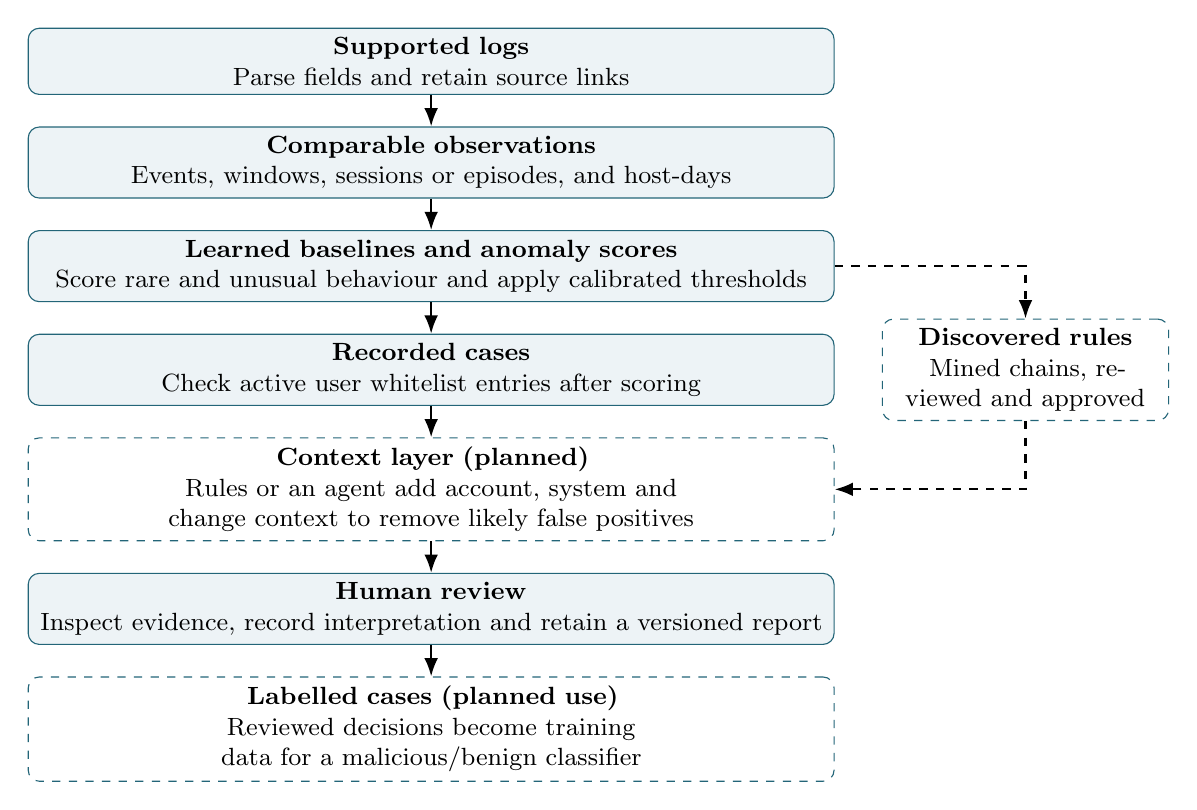
\begin{tikzpicture}[font=\small,>=Latex,
box/.style={draw=accent,fill=pale,rounded corners,align=center,text width=10cm,minimum height=0.75cm},
planned/.style={box,dashed,fill=white}]
\node[box] (logs) {\textbf{Supported logs}\\Parse fields and retain source links};
\node[box,below=0.4cm of logs] (observations) {\textbf{Comparable observations}\\Events, windows, sessions or episodes, and host-days};
\node[box,below=0.4cm of observations] (scores) {\textbf{Learned baselines and anomaly scores}\\Score rare and unusual behaviour and apply calibrated thresholds};
\node[box,below=0.4cm of scores] (known) {\textbf{Recorded cases}\\Check active user whitelist entries after scoring};
\node[planned,below=0.4cm of known] (context) {\textbf{Context layer (planned)}\\Rules or an agent add account, system and change context to remove likely false positives};
\node[box,below=0.4cm of context] (review) {\textbf{Human review}\\Inspect evidence, record interpretation and retain a versioned report};
\node[planned,below=0.4cm of review] (labels) {\textbf{Labelled cases (planned use)}\\Reviewed decisions become training data for a malicious/benign classifier};
\node[planned,text width=3.4cm,right=0.6cm of known] (rules) {\textbf{Discovered rules}\\Mined chains, reviewed and approved};
\draw[->,thick,dashed] (scores.east) -| (rules.north);
\draw[->,thick,dashed] (rules.south) |- (context.east);
\draw[->,thick] (logs)--(observations);
\draw[->,thick] (observations)--(scores);
\draw[->,thick] (scores)--(known);
\draw[->,thick] (known)--(context);
\draw[->,thick] (context)--(review);
\draw[->,thick] (review)--(labels);
\end{tikzpicture}
\caption{The evidence-to-review flow. Dashed boxes are planned; rule discovery is an added benefit whose mined candidates would feed the context layer only after review and approval. Whitelisting changes attention after scoring; neither a statistical finding nor a context layer supplies a security verdict.}
\label{fig:core-workflow}
\end{figure}

\subsection{The Four-Step Simple Workflow}

\begin{enumerate}
\item \textbf{Upload.} Paste lines or select a supported file. The console detects the source and shows parsing coverage; tabular exports require a raw-log column. When Phase 1 recognises fewer than 5\% of the sampled first lines, the workflow offers pattern discovery rather than implying that unknown data has been successfully analysed.
\item \textbf{Analyze.} Apply saved preprocessing and models. The result identifies findings worth attention; an active account exception can instead produce a \emph{Whitelisted} status. Uploading does not retrain the baseline.
\item \textbf{Map.} Place uploaded observations near comparable historical behaviour. This provides investigation context. Map geometry and group membership do not establish maliciousness.
\item \textbf{Review.} Retain the upload and inspect its chronological excerpt context. A reviewer records a label and supporting note. Assignment is recorded locally; opening a mail draft does not establish that a notification was delivered.
\end{enumerate}

\textbf{Illustrative example.} An operator asks about an authentication excerpt containing repeated failed logins. The analyst checks coverage, examines a flagged finding and reads the preceding and following uploaded lines. If those lines do not establish hostile activity, the analyst can record \emph{suspicious} or \emph{insufficient evidence} and identify the missing context. The example describes the workflow; actual flags, counts and placement must be verified on the supplied excerpt.

\subsection{Retaining Knowledge}

Human Review uses five dispositions: security relevant, suspicious, operationally interesting, expected behaviour and insufficient evidence. A decision on a historical group remains a group decision; uploaded findings have their own review context. These records are distinct from a whitelist override, and they are the starting material for the classifier goal (Section~\ref{sec:core-classifier}).

Reports connect findings, retained evidence and commentary to a case identifier. Each successful save preserves an application-level version with actor, time and digest; Word, PDF and HTML exports use saved evidence. A reviewed item's notes can start a report directly: its particulars fill the report and the notes become its analyst comments, exactly as typed. Optional ATT\&CK mappings describe behaviour but do not prove malice \cite{ref10}. This workflow retains investigation knowledge, while the validated label-export-to-training feedback loop remains unfinished.

The complete operating guide and screenshots are in companion Appendix~J. Detailed implementation and workflow semantics are in Appendix~I.

\clearpage
\section{Detection Approach}

The detection approach is unsupervised. It learns from unlabelled historical logs what is usual for each source, host and view, and ranks departures from that reference. No rule describing an attack is written in advance; known context enters afterwards, through recorded cases and, in future, a context layer.

Figure~\ref{fig:core-blocks} shows how one observation passes through the approach, as five blocks and the smaller blocks inside each. The subsections that follow describe them in turn.

\begin{figure}[H]
\centering
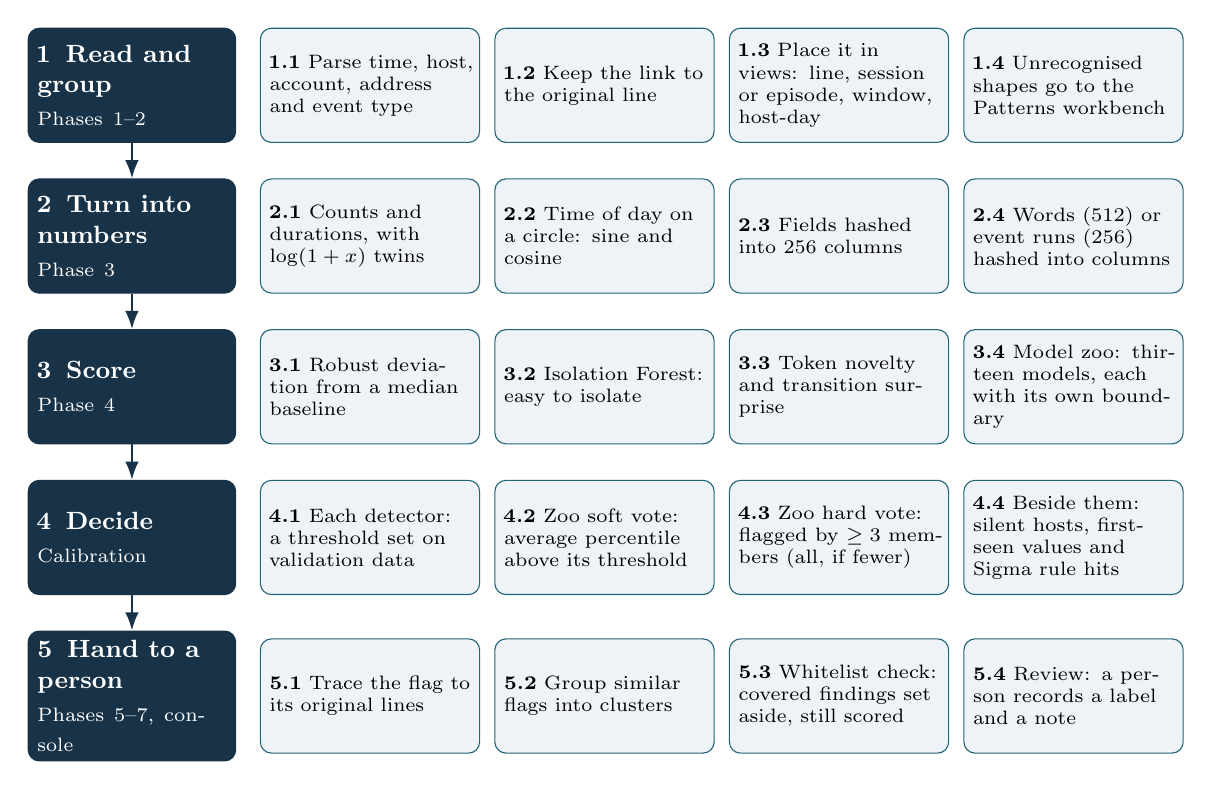
\begin{tikzpicture}[font=\scriptsize,>=Latex,node distance=0.18cm,
stage/.style={draw=ink,fill=ink,text=white,rounded corners,align=left,text width=2.4cm,minimum height=1.45cm,font=\small\bfseries},
part/.style={draw=accent,fill=pale,rounded corners,align=left,text width=2.55cm,minimum height=1.45cm}]
\node[stage] (s1) {1\enspace Read and group\\[1pt]{\scriptsize\mdseries Phases 1--2}};
\node[part,right=0.3cm of s1] (s11) {\textbf{1.1} Parse time, host, account, address and event type};
\node[part,right=of s11] (s12) {\textbf{1.2} Keep the link to the original line};
\node[part,right=of s12] (s13) {\textbf{1.3} Place it in views: line, session or episode, window, host-day};
\node[part,right=of s13] (s14) {\textbf{1.4} Unrecognised shapes go to the Patterns workbench};
\node[stage,below=0.45cm of s1] (s2) {2\enspace Turn into numbers\\[1pt]{\scriptsize\mdseries Phase 3}};
\node[part,right=0.3cm of s2] (s21) {\textbf{2.1} Counts and durations, with $\log(1+x)$ twins};
\node[part,right=of s21] (s22) {\textbf{2.2} Time of day on a circle: sine and cosine};
\node[part,right=of s22] (s23) {\textbf{2.3} Fields hashed into 256 columns};
\node[part,right=of s23] (s24) {\textbf{2.4} Words (512) or event runs (256) hashed into columns};
\node[stage,below=0.45cm of s2] (s3) {3\enspace Score\\[1pt]{\scriptsize\mdseries Phase 4}};
\node[part,right=0.3cm of s3] (s31) {\textbf{3.1} Robust deviation from a median baseline};
\node[part,right=of s31] (s32) {\textbf{3.2} Isolation Forest: easy to isolate};
\node[part,right=of s32] (s33) {\textbf{3.3} Token novelty and transition surprise};
\node[part,right=of s33] (s34) {\textbf{3.4} Model zoo: thirteen models, each with its own boundary};
\node[stage,below=0.45cm of s3] (s4) {4\enspace Decide\\[1pt]{\scriptsize\mdseries Calibration}};
\node[part,right=0.3cm of s4] (s41) {\textbf{4.1} Each detector: a threshold set on validation data};
\node[part,right=of s41] (s42) {\textbf{4.2} Zoo soft vote: average percentile above its threshold};
\node[part,right=of s42] (s43) {\textbf{4.3} Zoo hard vote: flagged by $\geq 3$ members (all, if fewer)};
\node[part,right=of s43] (s44) {\textbf{4.4} Beside them: silent hosts, first-seen values and Sigma rule hits};
\node[stage,below=0.45cm of s4] (s5) {5\enspace Hand to a person\\[1pt]{\scriptsize\mdseries Phases 5--7, console}};
\node[part,right=0.3cm of s5] (s51) {\textbf{5.1} Trace the flag to its original lines};
\node[part,right=of s51] (s52) {\textbf{5.2} Group similar flags into clusters};
\node[part,right=of s52] (s53) {\textbf{5.3} Whitelist check: covered findings set aside, still scored};
\node[part,right=of s53] (s54) {\textbf{5.4} Review: a person records a label and a note};
\draw[->,thick,draw=ink] (s1) -- (s2);
\draw[->,thick,draw=ink] (s2) -- (s3);
\draw[->,thick,draw=ink] (s3) -- (s4);
\draw[->,thick,draw=ink] (s4) -- (s5);
\end{tikzpicture}
\caption{How one observation becomes a flag. Each dark block is a step; the pale blocks are what it does. A flag can come from one detector (4.1), from the model zoo's consensus (4.2, 4.3) or from a Sigma rule for a known pattern (4.4); none of these is a security verdict, which only the review in 5.4 records.}
\label{fig:core-blocks}
\end{figure}

\subsection{Preprocessing and Feature Engineering}

Parsing turns a raw line into fields such as time, host, account, address and event type while preserving its provenance. The same events can then support different observations: one message, a five-minute host window, an authentication session or agent episode, or a host-day. These views answer different questions, so their alert counts cannot be treated as interchangeable incident counts.

Features describe \emph{how much}, \emph{who or what}, and \emph{when and in what order}. Examples are failed-login counts, session duration, account and event categories, periodic time and event-type fragments. Count transformations reduce the pull of very large values; training-fitted scaling preserves the reference. Hashing bounds feature dimensions but can merge distinct tokens into the same column (Section~\ref{sec:core-vectors}).

Unknown formats are surfaced in a Patterns workbench that groups line shapes and helps a person draft and test parser rules. Accepted workbench rules require manual adoption into Phase 1 before Analyze uses them. Recognising a line does not establish the security meaning of its content.

\subsection{From Raw Text to Numbers}\label{sec:core-vectors}

Anomaly models compare numbers, so every observation becomes one row of numbers before any model sees it. Phase 3 builds that row in five steps, in the same way for every observation and every split.

\begin{enumerate}[leftmargin=*]
\item \textbf{Normalise the text.} Addresses, numbers, hexadecimal values and key fingerprints in a message become placeholders such as \tok{{ip}} and \tok{{number}}, and the text is lower-cased, so that the same kind of message from two addresses reads alike.
\item \textbf{Split it into tokens.} Each categorical field becomes a \tok{column=value} token, such as \tok{event_type=ssh_login_failed}. The message of a single line contributes its words and adjacent word pairs (OSSEC: character sequences of three to five characters). A session, episode or window contributes its ordered event types as runs of one to three consecutive events.
\item \textbf{Hash the tokens into columns.} Each token passes through the MurmurHash3 function, and the remainder after dividing by the block's width \(m\) chooses its column. A column counts the tokens that land in it, and the block is scaled to unit length \cite{ref26}. Any token, including one never seen in training, receives a column without a fitted vocabulary, which is what lets novelty detection notice it.
\item \textbf{Describe the amounts.} Counts, rates and durations are kept together with a \(\log(1+x)\) twin, the time of day is placed on a circle as a sine and a cosine, and every numeric column is scaled with training statistics only.
\item \textbf{Concatenate.} One AUTH line becomes \(17+256+512=785\) numbers; one AUTH session becomes \(61+256+256=573\). Companion Appendix~H gives every view's blocks.
\end{enumerate}

\textbf{What 256 and 512 mean.} They are the number of columns \(m\) given to each hashed block: 256 for the categorical fields and for the runs of event types, and 512 for the words of a single line. They are settings of the vectoriser, chosen in advance, not parameters learned from the data. A larger \(m\) spreads the tokens over more columns, so fewer distinct tokens share one; a smaller \(m\) gives shorter rows and faster models. With \(k\) distinct tokens hashed uniformly into \(m\) columns, the share of tokens that share their column with another is about \(1-e^{-(k-1)/m}\). Free text has the largest vocabulary, so it receives the most columns; powers of two are a convention. Table~\ref{tab:core-hashwidth} compares this prediction with the AUTH data.

\begin{table}[H]
\centering\small
\begin{tabular}{lrrrrr}
\toprule
\textbf{AUTH block} & \textbf{Columns \(m\)} & \textbf{Distinct tokens \(k\)} & \textbf{\(k/m\)} & \textbf{Shared, predicted} & \textbf{Shared, measured} \\
\midrule
Categorical fields & 256 & 114 & 0.45 & 35.7\% & 42.1\% \\
Message words and pairs & 512 & 548 & 1.07 & 65.7\% & 66.8\% \\
Session event runs & 256 & 2,422 & 9.46 & 100.0\% & 100.0\% \\
\bottomrule
\end{tabular}
\caption{Share of distinct tokens that share their column with another token. Measured with Phase 3's own hashing on the first million AUTH events (fields and words) and on all 9.5 million AUTH sessions (event runs).}
\label{tab:core-hashwidth}
\end{table}

The session event-run block is saturated: every one of its 256 columns holds several runs, so it carries blurred information. Raising that width to 4,096 would lower the shared share to about 43\%, at the cost of wider rows and a re-run of Phases 3 and 4. Frequent tokens matter most and collide less often with each other, but a shared column can hide a rare token behind a common one; this is one reason a novelty finding can be missed (Section~\ref{sec:core-novelty}).

\subsection{Complementary Models}

No single definition of unusualness covers every security question. The application combines the perspectives in Table~\ref{tab:core-detectors}, supplemented by a model zoo of thirteen families (Section~\ref{sec:core-zoo}). Each learns its reference from the training period rather than from a rule. Rules for known attack patterns are checked beside them, as a separate fifth detector (Section~\ref{sec:core-sigma}).

\begin{table}[H]
\centering\small
\begin{tabular}{p{0.25\linewidth}p{0.66\linewidth}}
\toprule
\textbf{Perspective} & \textbf{Question answered} \\
\midrule
Robust deviation & Did a normally stable numerical feature move far from its resistant baseline? \\
Isolation Forest & Is this combination of features comparatively easy to isolate? \\
Token novelty & Does this observation activate features that were rare or absent in training? \\
Transition surprise & Is the next event uncommon after the previous event on this host? \\
\bottomrule
\end{tabular}
\caption{Complementary reasons to prioritise an observation. These are statistical questions, not estimates of attack probability.}
\label{tab:core-detectors}
\end{table}

Isolation Forest separates unusual combinations through random partitions \cite{ref3}. The model zoo adds families built on other principles; feature selection and screening help avoid unusable inputs or model behaviour.

\subsection{The Model Zoo: Many Assumptions Instead of One}\label{sec:core-zoo}

Every anomaly detector carries an assumption about what normal data look like: one compact cloud, a few clusters, a smooth region, independent features or a low-dimensional structure. When the assumption fits, the detector separates the unusual cleanly; when it does not, it flags the wrong observations with the same confidence. Nothing is known in advance about the shape of these log features, and without labels no assumption can be tested directly. The study therefore commits to none. It fits a \emph{zoo} of thirteen well-known families whose behaviour is easy to reason about, and asks two empirical questions: does combining them raise the proxy detection rate at the same alert budget, and where do they agree? Table~\ref{tab:core-zoo} groups the families by the mathematical principle each rests on.

\begin{table}[H]
\centering\small
\begin{tabular}{p{0.19\linewidth}p{0.33\linewidth}p{0.40\linewidth}}
\toprule
\textbf{Principle} & \textbf{Families} & \textbf{An observation counts as normal when it} \\
\midrule
Random partitioning & Isolation Forest \cite{ref3} & needs many random axis-parallel cuts to be isolated \\
Support boundary & One-class SVM with an RBF kernel \cite{ref23}; linear one-class SVM trained by SGD; elliptic envelope & lies inside a smooth surface, a hyperplane or a robust ellipse around the training data \\
Density and likelihood & Gaussian mixture; local outlier factor \cite{ref22}; HBOS \cite{ref24} & lies in a dense region: under a mixture of Gaussians, compared with its neighbours, or in each feature's histogram \\
Distance & \(k\)-nearest-neighbour distance; \(k\)-means distance & lies close to training observations, or to one of a few centres \\
Tail probability & ECOD \cite{ref25} & is not in the extreme tail of any single feature \\
Reconstruction & PCA; truncated SVD; autoencoder & can be rebuilt from a few linear or non-linear directions with little error \\
\bottomrule
\end{tabular}
\caption{The thirteen model-zoo families by principle. Once its threshold is set, each draws a boundary around normal behaviour in feature space; the shapes differ.}
\label{tab:core-zoo}
\end{table}

Most of these models can be read as drawing a boundary around normal behaviour: once a model's threshold is set, whatever lies outside it is flagged. The boundaries differ in shape (axis-parallel boxes for random cuts, a smooth closed surface for the RBF one-class SVM, an ellipse for the elliptic envelope, balls around centres for \(k\)-means, a band around a plane for reconstruction), and so do their mistakes: an observation can fall just outside one shape and well inside another. An observation outside several boundaries of different shapes is unusual in several distinct senses.

\textbf{Consensus design.} The zoo combines its members in two ways, both with equal weights:
\begin{itemize}[leftmargin=*]
\item \textbf{Common scale.} Each member's score is replaced by its percentile among that member's own training scores, so scores in different units become comparable.
\item \textbf{Soft vote (score averaging).} The ensemble score is the mean of the members' percentiles. It is thresholded in the same way as a single detector.
\item \textbf{Hard vote (\(k\)-out-of-\(n\)).} Each member flags with its own threshold, set on validation data at the 99.5th percentile of its scores within an alert cap. An observation is a consensus alert when at least three members flag it, or every member when fewer than three remain.
\end{itemize}
Learned weights or a stacked combiner would need labels and are not used. Membership is decided on validation data only. Models whose scores fail, that produce too few alerts, drift within the validation period, agree with no other model, or duplicate a kept model's ranking are removed. A greedy forward selection then keeps the shortest list of at least two members that comes within 0.005 of the best proxy detection rate; its curve records how much each added member helped. In the current runs most ensembles keep two members, so their consensus means that both agree (Appendix~H).

\textbf{Why agreement is informative.} Suppose two members raise false alarms on normal observations at rates \(f_1\) and \(f_2\), and do so independently. Both then raise one on the same normal observation at rate \(f_1f_2\): two members at 0.5\% each coincide on about one normal observation in 40,000. An observation that genuinely departs from both members' notions of normal is still flagged by each. Agreement therefore concentrates true statistical anomalies more than proportionately, and the more so the less the members' mistakes are correlated. This is why the zoo deliberately mixes principles, and why screening removes near-duplicate rankings, which would count one opinion twice, and isolated alert sets, which agree with nothing \cite{ref21,ref20}. The argument rests on independence, which is only approximate. Every member sees the same features, so all can share a blind spot, such as an attack that is ordinary in every feature, or tokens merged by hashing. Agreement raises confidence that an observation is statistically unusual; it does not establish that it is malicious.

\textbf{Weak, untuned members.} In supervised learning, settings such as the number of trees or the width of a kernel are tuned against labelled outcomes. This task has no labels, so there is no objective to tune against, and internal label-free criteria rarely beat sound defaults \cite{ref16}. Each family therefore runs with standard, fixed settings: for example 300 trees, \(\nu=0.05\), 35 neighbours, 8 mixture components, 32 centres and 20 histogram bins. An ensemble does not need any single member to be well tuned. Like the weak learners of ensemble learning, each member only needs to rank some unusual observations above normal ones, and combining diverse, imperfect rankings averages out their individual misfit. The proxy detection rate is used to choose members, never to tune a member's settings.

\textbf{Extending the zoo.} A new family needs one function that fits on the training rows and returns scores for the three splits. The same screening and selection then decide, on validation data alone, whether it joins the ensemble, and record why when it does not. Families better suited to these logs, such as sequence-aware models, can therefore be added without redesigning the combination.

\subsection{Novelty and Repeated New Behaviour}\label{sec:core-novelty}

Token novelty compares active retained features with their \textbf{fixed training presence counts}. It considers rare features as well as features absent from training, and uses the rarest active feature to score an observation. It does not merely compare complete log lines against a list of previously seen strings.

Suppose \tok{backup} is common in training and a feature associated with \tok{maint1} is absent. Table~\ref{tab:core-novelty} illustrates a later account change on the same host. A new maintenance account is one possible explanation; an unexpected login is another.

\begin{table}[H]
\centering\small
\begin{tabular}{lll}
\toprule
\textbf{Time} & \textbf{Illustrative activity on one host} & \textbf{Reading} \\
\midrule
08:00:00 & \tok{backup}: public-key login & Familiar account \\
08:00:03 & \tok{backup}: disconnect & Context \\
08:05:00 & \tok{backup}: public-key login & Familiar account \\
08:05:03 & \tok{backup}: disconnect & Context \\
\rowcolor{reviewred!7}
\textcolor{reviewred}{\textbf{08:10:00}} & \textcolor{reviewred}{\textbf{\tok{maint1}: public-key login}} & \textcolor{reviewred}{\textbf{Candidate for review}} \\
08:10:03 & \tok{maint1}: disconnect & Context \\
\bottomrule
\end{tabular}
\caption{Chronological explanation of a possible novelty finding. Red indicates attention. The example assumes a retained rare feature; it is not a measured result or proof of an attack.}
\label{tab:core-novelty}
\end{table}

If \tok{maint1} appears 100 times during testing, those repetitions do not update the fitted training counts. Each observation can still score highly and can flag against the saved threshold. Flags are not guaranteed: feature selection, encoding, hash collisions and calibration ties can conceal or exclude the distinction. A change already common in validation can affect the threshold before testing begins.

A regime change can therefore create sustained findings against an outdated reference. Review should establish the operational change before recalibration, retraining or a justified exception. Once review establishes that a repeated new behaviour is expected, it becomes a recorded case (a scoped whitelist entry, or a context rule once that layer exists) rather than a finding raised again each day. First-seen checks separately identify new accounts or addresses; they are not identical to hashed-feature rarity.

\subsection{Sequences, Sparse Sources and Maps}

Sequential mining discovers routines such as successful login, disconnect received and user disconnected. PrefixSpan describes frequent ordered subsequences \cite{ref4}; the implemented alert score separately measures the rarest host-conditioned next-event transition. A frequent routine is descriptive rather than a security policy, and a rare transition can be a legitimate operating change. Because routines are mined from the data rather than written by hand, they describe what the systems actually do; after review, a routine or a recurring exception to it can be proposed as a candidate rule for the context layer.

Sparse firewall sources use presence-oriented views rather than treating them as rich authentication-style baselines. Coverage and silence checks distinguish supported quiet periods from missing telemetry where the available evidence permits it. An empty file alone cannot establish that a system was healthy.

t-SNE and UMAP maps expose structure for exploration \cite{ref7,ref8}. New uploaded observations currently use saved higher-dimensional embeddings and neighbour-weighted placement on the retained map. This is an approximate placement, not a direct application of a saved final UMAP projector or a global linear mapping. An unfamiliar observation can appear near known behaviour; anomaly scores remain separate from map position.

\subsection{Rule Discovery as an Added Benefit}\label{sec:core-rules}

Beyond ranking observations, the mined structure can itself become detection knowledge. In the best case, a finding can be traced back to the chain or sequence of events that led to it, and a chain that recurs before findings later judged relevant can be developed into a rule. The current pipeline provides the raw material. Phase 4f mines frequent routines and 53 AUTH and 81 OSSEC sequential rules from the training period; one links \tok{SSH_DISCONNECT_RECEIVED} to a later \tok{SSH_USER_DISCONNECTED} with 100\% observed confidence over 5,493,782 training sessions. FP-growth alert profiles report attribute combinations over-represented among a detector's alerts \cite{ref5}, and each sequence finding names the unusual transition behind it.

Rules written by people tend to follow a heuristic, a guideline or a recognisable pattern. Mining has no such preference: it can surface a combination of event types, hosts, accounts and order that a person would not think to look for or would not find intuitive. That is the potential gain and also the risk. A pattern that is not intuitive is harder to justify, and it can reflect a logging artefact or one host's habits rather than security-relevant behaviour.

A mined pattern is therefore a candidate, not a rule. Frequency and confidence describe the training period; they supply no scope, severity, owner or expected response, and a broken routine does not imply compromise. A candidate becomes a rule only after an analyst gives it that meaning, it is replayed on later periods that include known maintenance, and it is approved; it can then join the rule-based part of the context layer or an operational monitoring platform. Tracing findings back to the chains that preceded real incidents also needs those incidents to be labelled. No mined rule has yet been adopted operationally. Companion Appendix~F lists every mined routine and rule.

\subsection{Known Patterns: Sigma Rules}\label{sec:core-sigma}

The statistical detectors rank what is rare, but some activity of concern is common and well described: repeated password guessing, spraying one password across many accounts, enumerating user names, or a firewall port scan. Such activity can be frequent in a busy environment and therefore unremarkable to a rarity score. The console therefore also runs detection rules written in the Sigma format, a vendor-neutral way of writing log detections \cite{ref28}. A rule matches single events by field tests; a correlation counts events or distinct values in a sliding window per group, or looks for several rules' events in order.

The enabled rules run over every analysed input and upload and over the historical validation and test periods. A hit flags the observations that hold its lines, Review lists any group holding such an observation whatever its rarity, and the Dashboard lists these items first. Rules change no model score, and a hit is a prompt for review, not a verdict. The two approaches answer different questions: rules find what people already know to look for, including common attacks; the statistical detectors find what is unusual whether or not anyone anticipated it. The eight starter rules (SSH guessing, spraying, enumeration and success after guessing, repeated \tok{su} failures, a stopped OSSEC agent, firewall port scans and sweeps) carry starting thresholds that need operational confirmation; Appendix~I describes the engine.

\subsection{Calibration and Postprocessing}

Observations are split chronologically into approximately 70\% training, 15\% validation and 15\% testing, with source/view-specific gaps at the boundaries. Training fits features and models; validation supports selection and thresholds; testing describes later behaviour under those fixed choices. Calibration targets apply per detector and view. They are not one global allowance or a guaranteed cap on every future day's workload.

\subsection{Recorded Cases: User Whitelisting}\label{sec:core-whitelist}

Rare activity that has already been examined and accepted should not request attention each time it recurs. \textbf{User whitelisting} records such cases and applies after scoring. Entries identify an exact, case-sensitive account on one server or all servers, with a required reason and optional inclusive expiry day. Addition and removal require the local administrator password and are audited; removed entries retain their history.

An observation is covered only if it names at least one account and every named account is actively covered on its corresponding server. A \tok{backup}/\tok{host-a} entry can cover its session; a session also naming unapproved \tok{root}, or one with no named account, remains uncovered. All flagged observations must be covered before a historical group is fully overridden.

Covered findings remain scored and retained but stop requesting attention. Saved uploads are evaluated against the current active list when read. This is an account-level exception: it can also cover failed logins naming that account, so scope and expiry matter. A \emph{Whitelisted} status is not a benign verdict. IP whitelisting is not implemented; Phase 9's approved-automation addresses provide separate interpretive context.

\subsection{Missing Context: Rule-Based and Agentic Filtering}\label{sec:core-context}

The detectors score behaviour against a statistical baseline. They have no access to the organisation's account directory, asset inventory, change records, maintenance calendar or knowledge of partner systems, so an observation that is unusual in the logs can be expected in context. A context layer between scoring and review is needed to remove such false positives before they consume analyst time.

Two forms are complementary. \emph{Rule-based} filters apply known, owned facts directly: an approved maintenance window, a registered service account or a permitted address range. They are transparent and cheap but limited to what has been written down. An \emph{agentic} layer gathers and weighs context for each finding, such as related events, recent changes and documented benign look-alikes of attacks, and proposes an interpretation with its reasons.

The current implementation contains starting points rather than this layer. Optional Phase~9 triage passes a finding, documented look-alikes and an approved-automation list to a local language model, which suggests a category; the approved-automation list is currently empty. Neither component is connected to account directories, inventories, change records or calendars, and neither removes findings automatically. Any future filtering decision should be recorded with its reason so that suppressed findings can be audited, as whitelist changes are.

\subsection{Explaining Flagged Groups: Hypotheses, Labels and Whitelisting}\label{sec:core-hypotheses}

The current priority is to explain the groups already flagged rather than to add detectors. For each group, analysts draft competing hypotheses: at least one benign explanation and one malicious alternative, each with the evidence that would confirm it and the observation that would refute it. This follows the analysis of competing hypotheses, which weighs evidence against every hypothesis and seeks evidence that rejects one, rather than gathering support for the first plausible story \cite{ref13}. Benign hypotheses start from the project's 31 documented look-alikes of attacks, and malicious ones from its 39 attack patterns.

A group leaves the review queue by one of two routes. It is \textbf{labelled} with one of the five dispositions when a hypothesis survives its test, or \emph{insufficient evidence} when none can yet be tested. It is \textbf{whitelisted} when a named account explains it and its recurring activity has been confirmed, with a server scope, a last day and a reason. Some explanations are a time window or an address rather than an account, and the whitelist cannot express them. They are recorded as approved change windows or approved automation addresses, the existing Phase~9 site context, alongside an \emph{expected behaviour} label. These records are the first rules of the context layer.

A first register, drafted on 16 October 2026 from the retained group summaries and recorded findings, holds 32 groups and 91 hypotheses; Table~\ref{tab:core-hypotheses} shows examples, and companion Appendix~M lists them all. Because the study year's raw lines were purged, most tests are questions to server, network and operational-technology owners and to change records, or a fresh upload of the same server's current logs. One answer often closes several groups. The effective SSH configuration of the mm servers could explain most of their concentration of alerts, and the owner of a job that runs daily at 07:01 could close at least five clusters.

\begin{table}[H]
\centering\small
\begin{tabular}{p{0.24\linewidth}p{0.2\linewidth}p{0.2\linewidth}p{0.24\linewidth}}
\toprule
\textbf{Flagged group} & \textbf{Benign hypothesis} & \textbf{Malicious alternative} & \textbf{Route if benign survives} \\
\midrule
mm06moc sessions at 07:01 each day & Scheduled job & Scheduled persistence or data transfer & Whitelist the job account on that server \\
mm servers with deprecated-option warnings & OpenSSH upgraded, old configuration kept & sshd configuration tampering & Label expected behaviour; fix the configuration \\
mm04kco root logins from a new internal address from 28 June & Change or migration run as root & Lateral movement with a valid account & Change window and label; never whitelist \tok{root} \\
mm03kco new cron messages from June & Cron job owned by a locked account & Cron persistence & Label operationally interesting \\
One IEC-104 telecontrol reset & Engineer's planned command & Unauthorised operational-technology command & Security relevant until the owner confirms \\
\bottomrule
\end{tabular}
\caption{Examples from the hypothesis register. Every group keeps its malicious alternative on record; none is resolved yet.}
\label{tab:core-hypotheses}
\end{table}

Explaining away carries its own risk: attackers imitate routine, and maintenance windows are good cover. A group is therefore explained only when its benign hypothesis survives the check that would refute it. The labels produced this way are what the classifier and the extensions in Section~\ref{sec:core-automl} need.

\subsection{Baselines for a Future Classifier}\label{sec:core-classifier}

Anomaly scores rank what is unusual; they do not estimate whether it is malicious. A malicious/benign classifier would, but it needs labelled examples, which do not yet exist. The current system builds towards it in three ways. The frozen runtime retains fitted preprocessing, feature definitions and detector baselines, so that future labels refer to consistently defined observations. Human Review records five dispositions, and reports retain the evidence behind each decision. Phase~8 provides label preparation and TF-IDF/SecureBERT classifier scaffolding.

No classifier has been trained, and exporting console labels for training is unfinished. Review labels need quality control before they are used as training data, and the chronological split should be kept so that a classifier is evaluated on periods after those it learns from. Anomaly scores can then serve as classifier inputs or as a baseline to compare against.

\subsection{AutoML as a Natural Extension}\label{sec:core-automl}

AutoML searches over model families, settings and ensembles against a validation objective. Mature systems combine that search with stacked ensembles, and AutoGluon had the highest average performance in a benchmark of nine frameworks \cite{ref14}. The model zoo already automates several of these steps without labels: feature selection, screening of unusable models and greedy forward ensemble selection against the proxy detection rate. Its hyperparameters are fixed per family, however, and its objective is a proxy, not attack detection.

Two extensions follow. Before labels exist, meta-learned methods select and tune unsupervised detectors from their performance on benchmark corpora \cite{ref15}. A large study found that label-free internal criteria rarely select better models than a sound default \cite{ref16}, so such tuning should be judged against reviewed outcomes rather than assumed to help. Once the hypothesis register yields labelled groups, supervised AutoML can build the decision model. A gradient-boosted classifier can use the observation features with the unsupervised anomaly scores as additional inputs \cite{ref17}, tuned and evaluated on the chronological split. Tabular foundation models are a candidate for the small labelled sets expected at first \cite{ref18}. In both cases the labels, not the search procedure, are the limiting resource.

Companion Appendix~G relates these components to the project's requirements. Appendix~H contains formulas, feature dimensions and detector selection details. Appendix~I contains sequence scoring, calibration, whitelist, local AI and other implementation semantics.

\clearpage
\section{Demonstrated Results}

\subsection{Historical Scope}

The recorded results describe one environment and a study year, not a multi-site benchmark. Table~\ref{tab:core-corpus} summarises the historical raw-line populations. The original corpus is no longer present in this workspace; these figures are retained results, not a new experiment.

\begin{table}[H]
\centering\small
\begin{tabular}{p{0.15\linewidth}r p{0.56\linewidth}}
\toprule
\textbf{Source} & \textbf{Raw lines} & \textbf{Interpretation} \\
\midrule
AUTH & 26,091,162 & Authentication-related activity dominates the corpus. \\
OSSEC & 115,288 & Agent operational messages, mainly connection and service behaviour. \\
PF & 3,955 & Packet records and batch-script lines; 41 active days. \\
IPFilter & 52,231 & Activity is confined to November 2025. \\
\bottomrule
\end{tabular}
\caption{Historical corpus described in the project README. Raw lines, constructed observations and incidents are different units.}
\label{tab:core-corpus}
\end{table}

\subsection{Complementary Findings}

The recorded sequence detector flagged \textbf{608 of 1,421,114 AUTH test sessions} (approximately 0.0428\%) and \textbf{19 of 4,417 OSSEC test episodes} (approximately 0.4302\%). These are candidate-observation fractions, not attack recall or false-positive rates.

Of the 608 AUTH sequence findings, \textbf{192 were not flagged by the other three mechanisms} in the Dashboard comparison: Isolation Forest, token novelty and model-zoo consensus. This shows complementary prioritisation on that population, obtained from a learned transition baseline rather than a hand-written rule. The nineteen OSSEC sequence findings all overlap token novelty, so incremental contribution is not uniform across sources.

Recorded investigation also found concentration around routine messages on busy hosts. Such concentration is useful evidence for checking the baseline and calibration, rather than proof of many separate attacks. Sources and complete reconstruction, threshold and overlap tables are retained in companion Appendix~K; the evidence register is Appendix~A.

\subsection{Implemented Capability}

The application demonstrates supported-log analysis, map placement, human review, versioned reporting and a workbench for unfamiliar formats. On 12 October 2026, the eight existing whitelist tests passed using isolated temporary stores, exercising matching, expiry, audit/removal records and retained-upload behaviour. These checks establish software behaviour under test conditions, not cybersecurity detection quality.

By 26 October 2026 the console also offered: Sigma rules as a fifth detector, written in a form by default or drafted from a plain-English description by the local model (a proof of concept, tested against a stand-in model), each tested on data before it can be accepted and stamped with who added it and when; a Dashboard that leads with what needs a decision and the next items to open, with a layout the analyst can rearrange, extend with their own read-only SQL tables (kept until refreshed) and tiles, and pack tightly; reports started from a reviewed item's notes, with HTML export; a menu grouped by investigation stage; and a hardened local service, in which only the console's own page can call the interface, queries need a separate SQL password, the page runs only its own scripts and cannot be framed, crafted workbooks and long lines are bounded, and exports cannot carry spreadsheet formulas or code (Appendix~I). Review's filters stop at a time limit set in Settings (120 seconds by default). All 229 automated tests of the console passed, including request-level checks of these protections. A rule-only parser for fixed-width event logs, with device classification, has 77 tests of its own and is not yet part of the pipeline run (Appendix~E).

The strongest demonstrated outcome is the connection between a statistical finding, its available evidence and a recorded analyst judgement. No new training or attack-validation experiment was performed when preparing this edition. Lead time before incidents, measured analyst time savings, independently validated precision/recall, the effect of a context layer and production rule-deployment effectiveness remain to be established.

\clearpage
\section{Limitations and Operational Acceptance}

\subsection{Evidence and Interpretation}

The project lacks an independently adjudicated malicious/benign dataset. Proxy-positive event types help inspect model behaviour but cannot establish attack recall, precision or false-negative rates. Review labels require quality control before use as learning labels. Quiet attacks that resemble ordinary activity may not be prioritised at all; living-off-the-land activity, which uses valid accounts and built-in tools, is the largest example (Section~\ref{sec:core-conclusion}).

Other limits include baseline contamination, concept drift, missing account, system and maintenance context (Section~\ref{sec:core-context}), hash collisions, heuristic session boundaries and uncertain event ordering. Model agreement and two-dimensional separation do not supply a security verdict. Whitelisting deliberately removes attention from covered accounts and can suppress genuinely concerning behaviour; it needs justified scope, expiry and review.

\subsection{Current Evidence Availability}

The frozen runtime retains fitted preprocessing, detector and model-zoo artifacts, maps, group summaries and selected caches. New supported uploads can be scored and retain their own excerpt evidence. Historical SQL, member-line and surrounding-event queries cannot recover purged source lines. Exact historical whitelist coverage also requires retained account facts and fails closed when those facts are unavailable.

The runtime omits raw lines, accounts and addresses from its package, but this does not imply that separate uploads, reports, console stores or screenshots contain none. The retained runtime is an inference baseline, not a complete reproducible training archive. Local execution still requires appropriate access control, retention, endpoint protection and recoverability.

\subsection{Acceptance Gates}

Before relying on the workbench operationally, a pilot should:
\begin{enumerate}
\item \textbf{Establish reviewed ground truth.} Resolve the hypothesis register's groups, and independently assess flagged and unflagged observations from later periods, including benign maintenance and controlled attack scenarios where appropriate.
\item \textbf{Measure detection and workload.} Report precision, recall, false alerts per host-day, review time and incremental benefit against the existing process, with explicit units and agreed targets.
\item \textbf{Measure lead time.} For incidents and significant operational problems in the pilot period, record whether and how early related observations were flagged, and how often flagged observations preceded nothing of concern.
\item \textbf{Integrate and audit context.} Connect a first rule-based or agentic context layer, record each filtering decision with its reason, and measure how many findings it removes and whether any removed finding was later judged relevant.
\item \textbf{Test discovered rules.} Replay mined candidate rules on held-out months, including maintenance; record how many survive review and approval, their alert volume, and whether any non-obvious candidate finds relevant activity that existing rules miss.
\item \textbf{Test change and missing data.} Exercise drift, new accounts, partial uploads, collection gaps, whitelist expiry and removal, and parser coverage on unfamiliar formats.
\item \textbf{Complete operational governance.} Assign rule/model ownership and demonstrate replay, approval, deployment monitoring, rollback, identity integration and recovery.
\end{enumerate}

Optional local language-model assistance remains subject to evidence checking. A context layer connected to organisational sources, a validated maliciousness classifier, a completed review-to-training feedback loop and a governed production-rule registry are unfinished. The detailed acceptance matrix and recorded qualifications are retained in Appendix~K.

\clearpage
\section{Conclusion and Next Step}\label{sec:core-conclusion}

Project DAD Console is a working step from reacting to incidents towards discovering early signs of them. It learns normal behaviour from local logs, ranks rare and anomalous observations without relying on hand-written rules and keeps each finding connected to its evidence and a recorded human judgement. Already-recorded cases are handled by an explicit, audited user whitelist that preserves scores and retained findings. As an added benefit, the routines and sequential rules mined by the pipeline are a source of candidate rules, including ones a person might not think to write; none has yet been reviewed and adopted.

The historical sequence results demonstrate that a learned behavioural perspective can identify candidates missed by other mechanisms. They do not establish how many attacks were detected, how early, or how much analyst effort was saved. The current frozen runtime continues to support new supported uploads, while investigation of purged historical lines is unavailable.

\textbf{The largest blind spot: living off the land.} Many intrusions avoid malware and use what is already present instead: valid accounts and keys, SSH, \tok{su}, scheduled jobs and built-in administration tools \cite{ref27}. Such activity is a very large blind spot for this study, for four reasons.
\begin{enumerate}[leftmargin=*]
\item \textbf{It is designed to look common.} The detectors rank what is rare. A valid account logging in with its usual key, from a familiar source at an ordinary hour, is normal in every feature.
\item \textbf{The sources see little of it.} The four logs record logins, privilege changes, agent alerts and blocked packets, but largely not what is done inside a session, where most of this activity takes place.
\item \textbf{Use hides misuse.} The more an account is used, the more its misuse resembles its own baseline. Whitelisting an account deliberately removes it from attention, and the training period itself may already contain such activity, which then counts as normal.
\item \textbf{Careful operators leave little to notice.} Activity that stays within routine volumes, orders and sources gives the robust, sequence and first-seen checks nothing to flag.
\end{enumerate}
The absence of a flag is therefore not evidence that no attack took place. Closing this gap needs other evidence: command-level auditing on the servers, per-account baselines of sources, hosts and times, the context layer's knowledge of change windows and approved automation, and hypothesis-driven hunting mapped to ATT\&CK techniques such as the use of valid accounts \cite{ref10}.

A fifth source is being onboarded: a control system's fixed-width event log, read by a parser that applies only the owner's stated rules and sends everything else to an exceptions file, with devices classified by the states they show. Its observations, features and models remain to be decided. Two parts of the wider effort are not yet in place: a context layer that removes false positives using knowledge of the organisation's accounts and systems, and a malicious/benign classifier trained on reviewed labels. The immediate priority is the hypothesis register: explaining each flagged group so that it is either labelled or whitelisted, with its malicious alternative on record. The next step is an analyst-assisted pilot that measures lead time and workload on independently reviewed data, connects a first context layer and collects quality-controlled labels. With those labels, AutoML becomes a natural extension for tuning the detectors and building the decision model. Operational response should follow demonstrated evidence and ownership, rather than treating unusualness as an automatic decision.

\textbf{Companion reference.} The separately compiled \nolinkurl{TECHNICAL_WHITEPAPER_APPENDICES.tex} retains: A, evidence register; B, metric definitions; C, starting-draft changes; D, API; E, parsing patterns; F, mined routines; G, detailed requirements and technique reference; H, mathematical methods and feature reference; I, implementation and workflow detail; J, user guide and screenshots; K, detailed results and acceptance programme; L, application version history; and M, the hypothesis register for the recorded groups. The appendices have their own reference list and local cross-references.


\clearpage
\section{References}

\begingroup
\small
\renewcommand{\section}[2]{}
\begin{thebibliography}{10}
\bibitem{ref1} Stouffer, K., et al. (2023). \emph{Guide to Operational Technology (OT) Security}. NIST Special Publication 800-82 Revision 3. \href{\detokenize{https://doi.org/10.6028/NIST.SP.800-82r3}}{Publication and DOI}.
\bibitem{ref3} Liu, F. T., Ting, K. M., and Zhou, Z.-H. (2008). \emph{Isolation Forest}. IEEE International Conference on Data Mining, pp. 413--422. DOI: 10.1109/ICDM.2008.17. \href{\detokenize{https://cs.nju.edu.cn/zhouzh/zhouzh.files/publication/icdm08b.pdf}}{Author-hosted paper}.
\bibitem{ref4} Pei, J., Han, J., Mortazavi-Asl, B., Pinto, H., Chen, Q., Dayal, U., and Hsu, M.-C. (2001). \emph{PrefixSpan: Mining Sequential Patterns Efficiently by Prefix-Projected Pattern Growth}. IEEE International Conference on Data Engineering, pp. 215--224. \href{\detokenize{https://www.cs.sfu.ca/~jpei/publications/span.pdf}}{Author-hosted paper}.
\bibitem{ref5} Han, J., Pei, J., Yin, Y., and Mao, R. (2004). \emph{Mining Frequent Patterns without Candidate Generation: A Frequent-Pattern Tree Approach}. Data Mining and Knowledge Discovery, 8, pp. 53--87. \href{\detokenize{https://www.cs.sfu.ca/~jpei/publications/dami03_fpgrowth.pdf}}{Author-hosted paper}.
\bibitem{ref7} van der Maaten, L., and Hinton, G. (2008). \emph{Visualizing Data using t-SNE}. Journal of Machine Learning Research, 9(86), pp. 2579--2605. \href{\detokenize{https://jmlr.org/papers/v9/vandermaaten08a.html}}{Paper}.
\bibitem{ref8} McInnes, L., Healy, J., and Melville, J. (2018; revised 2020). \emph{UMAP: Uniform Manifold Approximation and Projection for Dimension Reduction}. arXiv:1802.03426. \href{\detokenize{https://arxiv.org/abs/1802.03426}}{Paper}.
\bibitem{ref10} MITRE. \emph{ATT\&CK Resources}. Official introduction to the adversary-behaviour knowledge base. \href{\detokenize{https://attack.mitre.org/resources/}}{Resource}.
\bibitem{ref13} Heuer, R. J., Jr. (1999). \emph{Psychology of Intelligence Analysis}, Chapter 8: Analysis of Competing Hypotheses. Center for the Study of Intelligence, Central Intelligence Agency. \href{\detokenize{https://www.cia.gov/resources/csi/static/Pyschology-of-Intelligence-Analysis.pdf}}{Publication}.
\bibitem{ref14} Gijsbers, P., Bueno, M. L. P., Coors, S., LeDell, E., Poirier, S., Thomas, J., Bischl, B., and Vanschoren, J. (2024). \emph{AMLB: an AutoML Benchmark}. Journal of Machine Learning Research, 25. \href{\detokenize{https://jmlr.org/papers/v25/22-0493.html}}{Paper}.
\bibitem{ref15} Zhao, Y., Rossi, R. A., and Akoglu, L. (2021). \emph{Automatic Unsupervised Outlier Model Selection}. Advances in Neural Information Processing Systems 34. \href{\detokenize{https://proceedings.neurips.cc/paper/2021/file/23c894276a2c5a16470e6a31f4618d73-Paper.pdf}}{Paper}.
\bibitem{ref16} Ma, M. Q., Zhao, Y., Zhang, X., and Akoglu, L. (2023). \emph{The Need for Unsupervised Outlier Model Selection: A Review and Evaluation of Internal Evaluation Strategies}. ACM SIGKDD Explorations. \href{\detokenize{https://www.andrew.cmu.edu/user/lakoglu/pubs/23-SigKDDExplor-UnsupervisedModelSelection-WhitePaperSurvey.pdf}}{Author-hosted paper}.
\bibitem{ref17} Zhao, Y., and Hryniewicki, M. K. (2018). \emph{XGBOD: Improving Supervised Outlier Detection with Unsupervised Representation Learning}. International Joint Conference on Neural Networks. arXiv:1912.00290. \href{\detokenize{https://arxiv.org/abs/1912.00290}}{Paper}.
\bibitem{ref18} Hollmann, N., et al. (2025). \emph{Accurate Predictions on Small Data with a Tabular Foundation Model}. Nature, 637, pp. 319--326. \href{\detokenize{https://pubmed.ncbi.nlm.nih.gov/39780007/}}{PubMed record}.
\bibitem{ref20} Aggarwal, C. C., and Sathe, S. (2017). \emph{Outlier Ensembles: An Introduction}. Springer. DOI: 10.1007/978-3-319-54765-7.
\bibitem{ref21} Zimek, A., Campello, R. J. G. B., and Sander, J. (2014). \emph{Ensembles for Unsupervised Outlier Detection: Challenges and Research Questions}. ACM SIGKDD Explorations Newsletter, 15(1), pp. 11--22. DOI: 10.1145/2594473.2594476.
\bibitem{ref22} Breunig, M. M., Kriegel, H.-P., Ng, R. T., and Sander, J. (2000). \emph{LOF: Identifying Density-Based Local Outliers}. ACM SIGMOD International Conference on Management of Data, pp. 93--104. DOI: 10.1145/342009.335388.
\bibitem{ref23} Sch\"olkopf, B., Platt, J. C., Shawe-Taylor, J., Smola, A. J., and Williamson, R. C. (2001). \emph{Estimating the Support of a High-Dimensional Distribution}. Neural Computation, 13(7), pp. 1443--1471. DOI: 10.1162/089976601750264965.
\bibitem{ref24} Goldstein, M., and Dengel, A. (2012). \emph{Histogram-based Outlier Score (HBOS): A Fast Unsupervised Anomaly Detection Algorithm}. KI-2012: Poster and Demo Track, pp. 59--63.
\bibitem{ref25} Li, Z., Zhao, Y., Hu, X., Botta, N., Ionescu, C., and Chen, G. H. (2022). \emph{ECOD: Unsupervised Outlier Detection Using Empirical Cumulative Distribution Functions}. IEEE Transactions on Knowledge and Data Engineering. arXiv:2201.00382. \href{\detokenize{https://arxiv.org/abs/2201.00382}}{Paper}.
\bibitem{ref26} Weinberger, K., Dasgupta, A., Langford, J., Smola, A., and Attenberg, J. (2009). \emph{Feature Hashing for Large Scale Multitask Learning}. International Conference on Machine Learning, pp. 1113--1120. arXiv:0902.2206. \href{\detokenize{https://arxiv.org/abs/0902.2206}}{Paper}.
\bibitem{ref27} Cybersecurity and Infrastructure Security Agency, National Security Agency, Federal Bureau of Investigation, and international partners (2024). \emph{Identifying and Mitigating Living Off the Land Techniques}. Joint cybersecurity guidance, February 2024.
\bibitem{ref28} SigmaHQ. \emph{Sigma Specification}: the generic, vendor-neutral signature format for log detections, its rules and correlation rules. \href{\detokenize{https://github.com/SigmaHQ/sigma-specification}}{Specification}.
\end{thebibliography}
\endgroup

External references support the methods and operational context. Project-specific claims are supported by the companion evidence register and detailed results; method citations do not validate this application's detection performance.

\end{document}
